\documentclass[tikz]{standalone}
\usetikzlibrary{patterns}
\usetikzlibrary{shapes,arrows}
\usetikzlibrary{decorations.pathreplacing, positioning}
\definecolor{greengreen}{rgb}{0.0, 0.42, 0.24}
\definecolor{calpolypomonagreen}{rgb}{0.12, 0.3, 0.17}
\definecolor{forestgreen}{rgb}{0.13, 0.55, 0.13}

\begin{document}
\noindent
  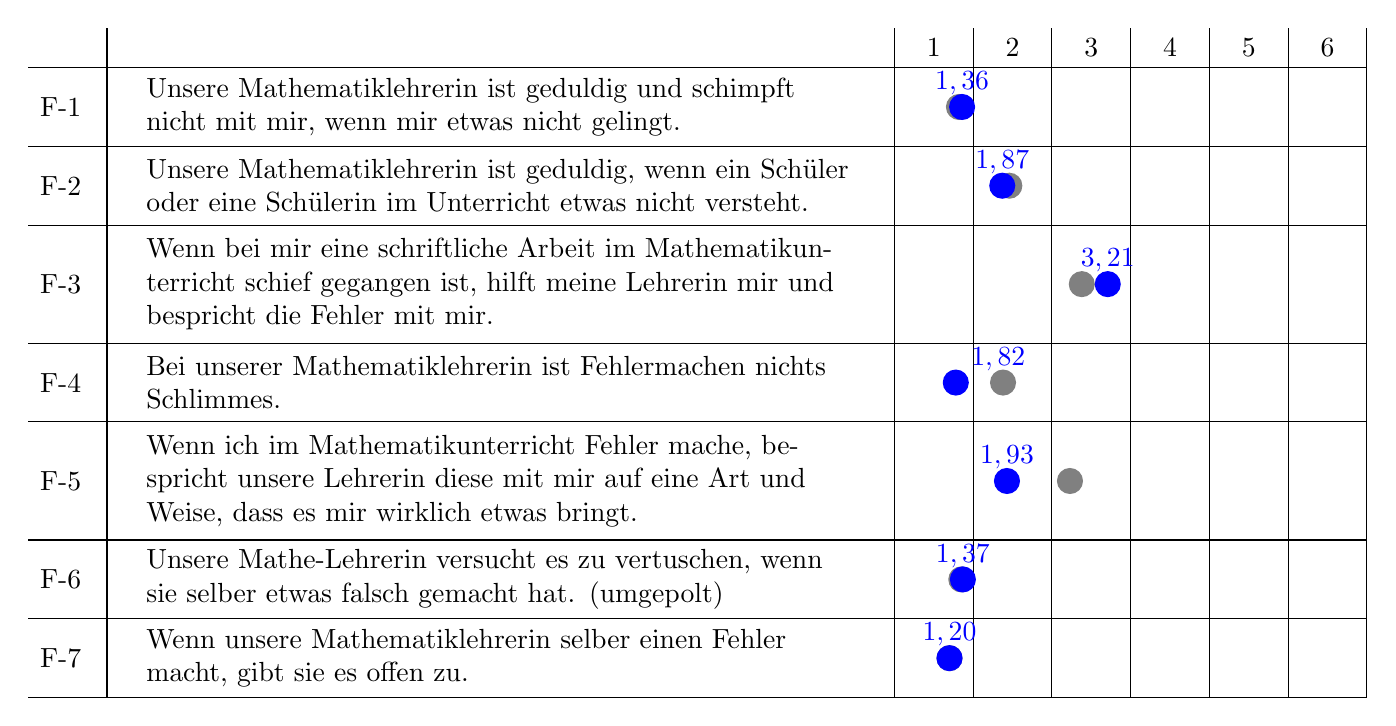
\begin{tikzpicture}

    \foreach \y in {0,1,2,3.5,4.5,6,7,8}
        \draw (-1, 0 - \y) -- (16, 0 - \y);
    \foreach \x in {0,10,11,12,13,14,15,16}
        \draw (0 + \x, 0.5) -- (0 + \x, - 8);
    
    \node at (10.5, 0.25) {$1$};
    \node at (11.5, 0.25) {$2$};
    \node at (12.5, 0.25) {$3$};
    \node at (13.5, 0.25) {$4$};
    \node at (14.5, 0.25) {$5$};
    \node at (15.5, 0.25) {$6$};

    \node[thick, align=left, text width=1cm] at (-0.35, -0.5) {F-1};
    \node[thick, align=left, text width=9cm] at (5, -0.5) {Unsere Mathematiklehrerin ist geduldig und schimpft nicht mit mir, wenn mir etwas nicht gelingt.};
    \node[thick, circle, fill=gray, minimum width=0.25] (1) at (9.5 + 1.32, -0.5) {};
    \node[thick, blue] at (9.5 + 1.36, -0.2) {$1,36$};
    \node[thick, circle, fill=blue, minimum width=0.25] (1) at (9.5 + 1.36, -0.5) {};


    \node[thick, align=left, text width=1cm] at (-0.35, -1.5) {F-2};
    \node[thick, align=left, text width=9cm] at (5, -1.5) {Unsere Mathematiklehrerin ist geduldig, wenn ein Schüler oder eine Schülerin im Unterricht etwas nicht versteht.};
    \node[thick, circle, fill=gray, minimum width=0.25] (2) at (9.5 + 1.96, -1.5) {};
    \node[thick, blue] at (9.5 + 1.87, -1.2) {$1,87$};
    \node[thick, circle, fill=blue, minimum width=0.25] (1) at (9.5 + 1.87, -1.5) {};


    \node[thick, align=left, text width=1cm] at (-0.35, -2.75) {F-3};
    \node[thick, align=left, text width=9cm] at (5, -2.75) {Wenn bei mir eine schriftliche Arbeit im Mathematikunterricht schief gegangen ist, hilft meine Lehrerin mir und bespricht die Fehler mit mir.};
    \node[thick, circle, fill=gray, minimum width=0.25] (3) at (9.5 + 2.88, -2.75) {};
    \node[thick, blue] at (9.5 + 3.21, -2.45) {$3,21$};
    \node[thick, circle, fill=blue, minimum width=0.25] (1) at (9.5 + 3.21, -2.75) {};


    \node[thick, align=left, text width=1cm] at (-0.35, -4) {F-4};
    \node[thick, align=left, text width=9cm] at (5, -4) {Bei unserer Mathematiklehrerin ist Fehlermachen nichts Schlimmes.};
    \node[thick, circle, fill=gray, minimum width=0.25] (4) at (9.5 + 1.88, -4) {};
    \node[thick, blue] at (9.5 + 1.82, -3.7) {$1,82$};
    \node[thick, circle, fill=blue, minimum width=0.25] (1) at (9.5 + 1.28, -4) {};


    \node[thick, align=left, text width=1cm] at (-0.35, -5.25) {F-5};
    \node[thick, align=left, text width=9cm] at (5, -5.25) {Wenn ich im Mathematikunterricht Fehler mache, bespricht unsere Lehrerin diese mit mir auf eine Art und Weise, dass es mir wirklich etwas bringt.};
    \node[thick, circle, fill=gray, minimum width=0.25] (5) at (9.5 + 2.73, -5.25) {};
    \node[thick, blue] at (9.5 + 1.93, -4.95) {$1,93$};
    \node[thick, circle, fill=blue, minimum width=0.25] (1) at (9.5 + 1.93, -5.25) {};


    \node[thick, align=left, text width=1cm] at (-0.35, -6.5) {F-6};
    \node[thick, align=left, text width=9cm] at (5, -6.5) {Unsere Mathe-Lehrerin versucht es zu vertuschen, wenn sie selber etwas falsch gemacht hat. (umgepolt)};
    \node[thick, circle, fill=gray, minimum width=0.25] (6) at (9.5 + 1.35, -6.5) {};
    \node[thick, blue] at (9.5 + 1.37, -6.2) {$1,37$};
    \node[thick, circle, fill=blue, minimum width=0.25] (1) at (9.5 + 1.37, -6.5) {};


    \node[thick, align=left, text width=1cm] at (-0.35, -7.5) {F-7};
    \node[thick, align=left, text width=9cm] at (5, -7.5) {Wenn unsere Mathematiklehrerin selber einen Fehler macht, gibt sie es offen zu.};
    \node[thick, circle, fill=gray, minimum width=0.25] (7) at (9.5 + 1.2, -7.5) {};
    \node[thick, blue] at (9.5 + 1.2, -7.2) {$1,20$};
    \node[thick, circle, fill=blue, minimum width=0.25] (1) at (9.5 + 1.2, -7.5) {};

    %\draw[color=blue, thick] (1) to (2) to (3) to (4) to (5);

  \end{tikzpicture}%
\end{document}
